% ----------------------------------------------------------------------
% Configurar a classe do documento
% ----------------------------------------------------------------------
\documentclass[12pt]{article}

% ----------------------------------------------------------------------
% Definir packages externos, língua, margens, tipos de letra, novos 
% comandos e cores
% ----------------------------------------------------------------------
\usepackage[utf8]{inputenc} % Codificação utilizada
\usepackage[english]{babel} % Idioma de escrita

\usepackage[export]{adjustbox} % Alinhar imagens
\usepackage{amsmath} % Comandos extra para escrita matemática
\usepackage{amssymb} % Símbolos matemáticos
\usepackage{anysize} % Personalizar as margens
    \marginsize{2cm}{2cm}{2cm}{2cm} % {esquerda}{direita}{cima}{baixo}
\usepackage{appendix} % Apêndices
\usepackage{cancel} % Cancelar expressões
\usepackage{caption} % Legendas
    \DeclareCaptionFont{newfont}{\fontfamily{cmss}\selectfont}
    \captionsetup{labelfont={bf, newfont}}
\usepackage{cite} % Citações, tipo [1 - 3]
\usepackage{color} % Colorir texto
\usepackage{fancyhdr} % Cabeçalho e rodapé
    \pagestyle{fancy}
    \fancyhf{}
    \fancyhead[L]{\footnotesize\fontfamily{cmss}\selectfont IST} % Esquerda do cabeçalho
    \fancyhead[R]{\footnotesize\fontfamily{cmss}\selectfont ULisboa} % Direita do cabeçalho
    \fancyfoot[L]{\footnotesize\fontfamily{cmss}\selectfont Robotics} % Esquerda do rodapé
    \fancyfoot[C]{\thepage} % Centro do rodapé
    \fancyfoot[R]{\footnotesize\fontfamily{cmss}\selectfont MEEC} % Direita do rodapé
    \renewcommand{\footrulewidth}{0.4pt} % Régua do rodapé
\usepackage{float} % Utilizar o especificador [H] nas figuras
\usepackage{graphicx} % Imagens em LaTeX
\usepackage[colorlinks = true, plainpages = true, linkcolor = istblue, urlcolor = istblue, citecolor = istblue, anchorcolor = istblue]{hyperref}
\usepackage{indentfirst} % Primeiro parágrafo
\usepackage{siunitx} % Unidades SI
\usepackage{subcaption} % Subfiguras
\usepackage{titlesec} % Tipo de letra
    \titleformat{\section}{\fontfamily{cmss}\selectfont\Large\bfseries}{\thesection}{1em}{}
    \titleformat{\subsection}{\fontfamily{cmss}\selectfont\large\bfseries}{\thesubsection}{1em}{}
    \titleformat{\subsubsection}{\fontfamily{cmss}\selectfont\normalsize\bfseries}{\thesubsubsection}{1em}{}
    \fancyfoot[C]{\fontfamily{cmss}\selectfont\thepage}

% Encher de texto aleatório (apagar)
\usepackage{lipsum}
\usepackage{duckuments}

% Novos e renovar comandos
\newcommand{\sen}{\operatorname{\sen}} % Definição da função seno
\newcommand{\HRule}{\rule{\linewidth}{0.5mm}} % Definição de uma régua
\renewcommand{\appendixpagename}{\LARGE \fontfamily{cmss}\selectfont Appendices}
\renewcommand{\appendixtocname}{Appendices}

% Cores
\definecolor{istblue}{RGB}{3, 171, 230}
\definecolor{dkgreen}{rgb}{0,0.6,0}
\definecolor{gray}{rgb}{0.5,0.5,0.5}

%%%%%%%%%%%%%%%%%%%%%%%%%%%%%%%%%%%%%%%%%%%%%%%%%%%%%%%%%%%%%%%%%%%%%%%%
%                               Documento                              %
%%%%%%%%%%%%%%%%%%%%%%%%%%%%%%%%%%%%%%%%%%%%%%%%%%%%%%%%%%%%%%%%%%%%%%%%
\begin{document}

% ----------------------------------------------------------------------
% Capa
% ----------------------------------------------------------------------
\begin{center}
    \begin{figure}
        \vspace{-1.0cm}
        
\includegraphics[scale = 0.3, left]{Imagens/IST_A.eps} % Tipo de assinatura do IST
    \end{figure}
    \mbox{}\\[2.0cm]
    \textsc{\Huge Robotics}\\[2.5cm]
    \textsc{\LARGE MEEC}\\[2.0cm]
    \HRule\\[0.4cm]
    {\large \bf {\fontfamily{cmss}\selectfont Orientation Estimation and Trajectory Analysis Using Sensor Data}}\\[0.2cm]
    \HRule\\[1.5cm]
\end{center}

\begin{flushleft}
    \textbf{\fontfamily{cmss}\selectfont Authors:}
\end{flushleft}

\begin{center}
    \begin{minipage}{0.5\textwidth}
        \begin{flushleft}
            Vladimiro Roque (98589)\\
            Lorem Ipsum (\texttt{ISTID} $\in \mathbb{Z}^+$)\\
            Lorem Ipsum (\texttt{ISTID} $\in \mathbb{Z}^+$)
        \end{flushleft}
    \end{minipage}%
    \begin{minipage}{0.5\textwidth}
        \begin{flushright}
            \href{mailto:vladimiro.roque@tecnico.ulisboa.pt}{\texttt{vladimiro.roque@tecnico.ulisboa.pt}}\\
            \href{mailto:lorem.ipsum@tecnico.ulisboa.pt}{\texttt{lorem.ipsum@tecnico.ulisboa.pt}}\\
            \href{mailto:lorem.ipsum@tecnico.ulisboa.pt}{\texttt{lorem.ipsum@tecnico.ulisboa.pt}}
        \end{flushright}
    \end{minipage}
\end{center}
    
\begin{flushleft}
    \large $\boxed{\text{\bf \fontfamily{cmss}\selectfont Group} \ \textbf{9}}$\\[4.0cm]
\end{flushleft}
    
\begin{center}
    \large \bf \fontfamily{cmss}\selectfont 2024/2025 -- 1º Semester, P2
\end{center}

\thispagestyle{empty}

\setcounter{page}{0}

\newpage

% ----------------------------------------------------------------------
% Conteúdo
% ----------------------------------------------------------------------
\tableofcontents 

\newpage

% ----------------------------------------------------------------------
% Desenvolvimento
% ----------------------------------------------------------------------
\section{Group Members Contribution} % Professor pediu esta seção, está nos slides da teorica (1º slides)


\lipsum[1] \cite{refs1}

\section{Introduction} 

%% Escrever..........................(não esquecer!)

\lipsum[1] \cite{refs2}

\lipsum[2-3]

\newpage

\section{Tasks}

\subsection{Task 1}

\subsubsection{Como apresentar uma só figura}

\begin{figure}[H]
	\begin{center}
 		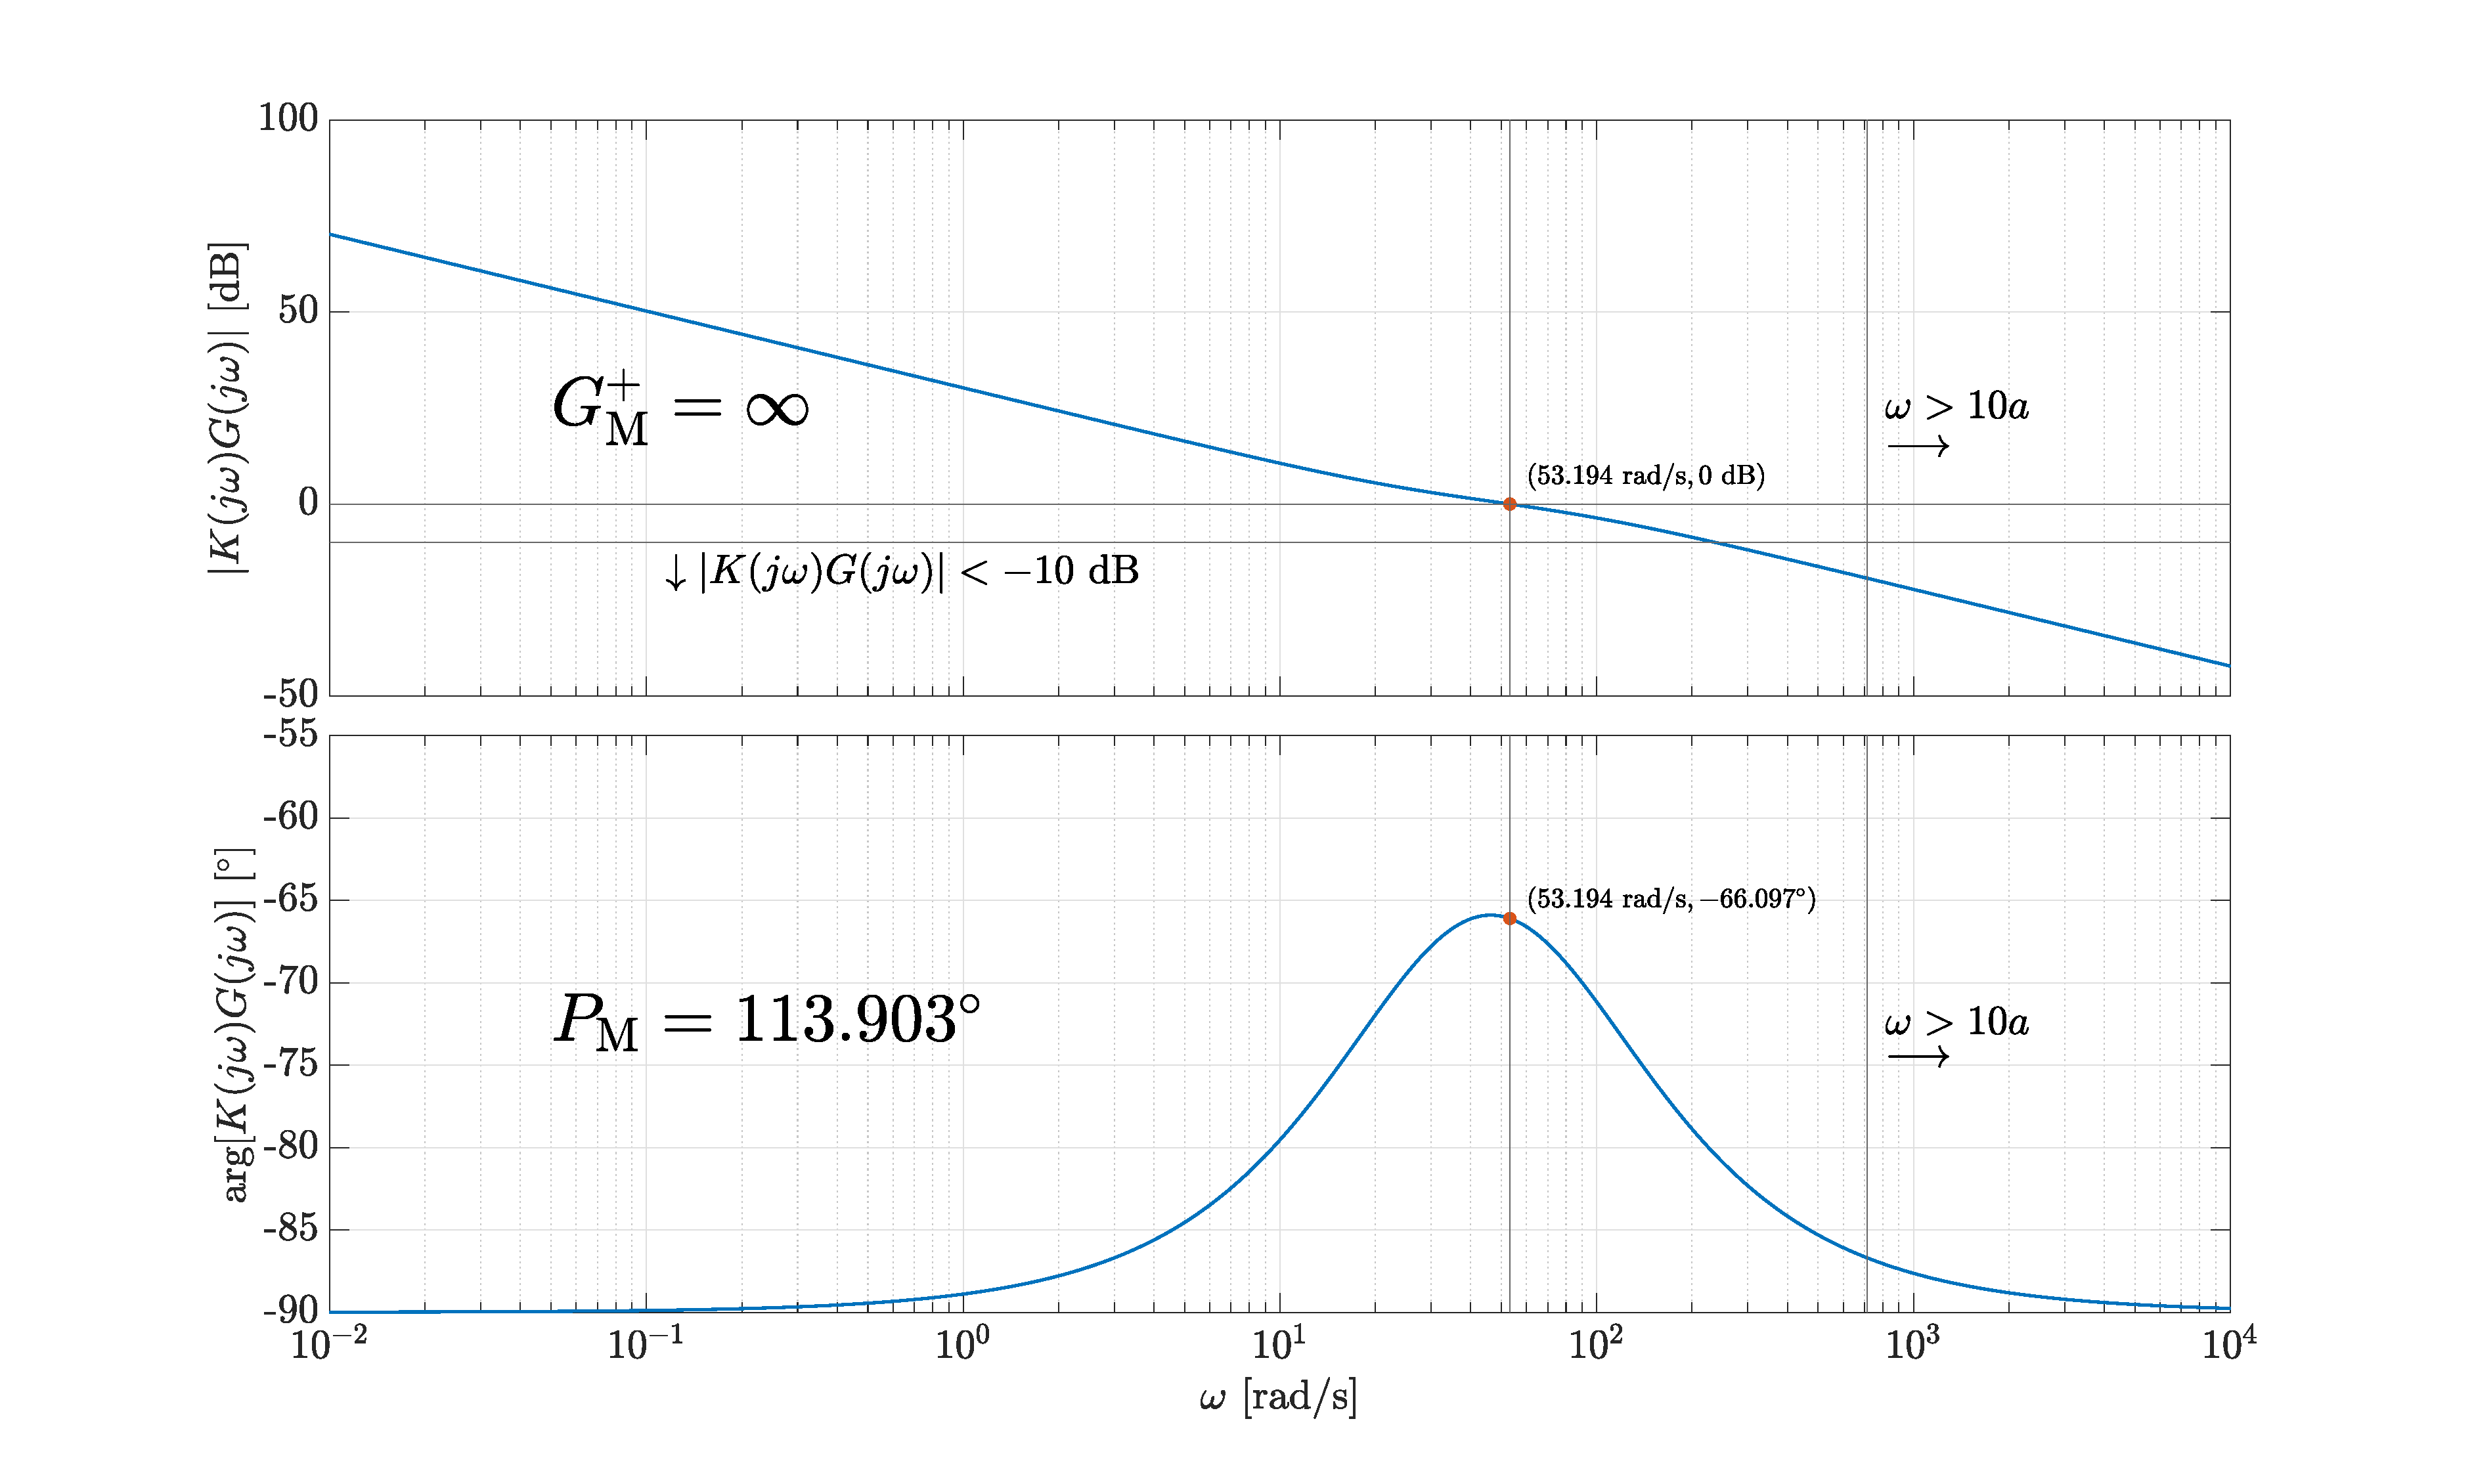
\includegraphics[width = 0.8\textwidth]{Imagens/Image.eps}
 		\caption{Descrição da imagem}
 		\label{fig:1}
	\end{center} 
\end{figure}

\subsubsection{Como apresentar subfiguras}

\begin{figure}[H]
    \centering
    \begin{subfigure}{0.33\textwidth}
        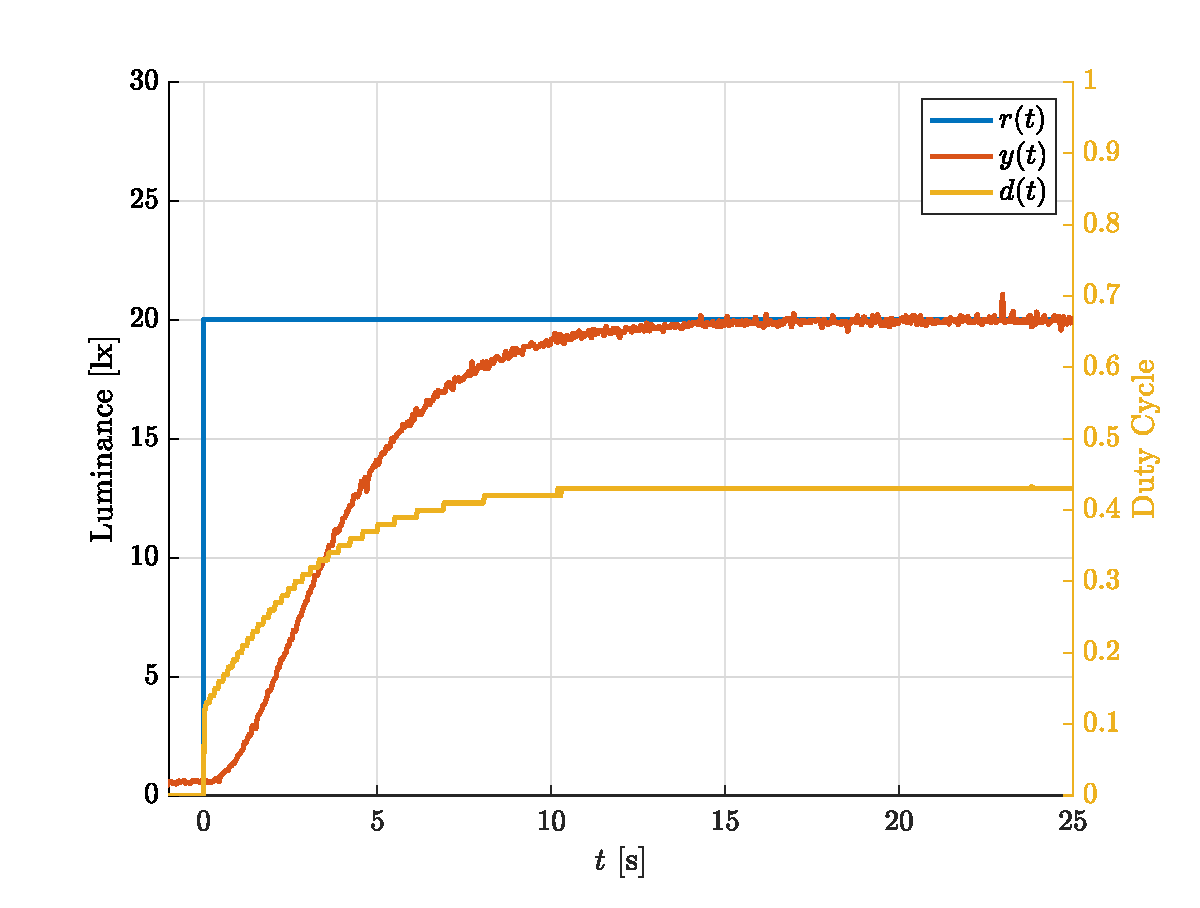
\includegraphics[width=\linewidth]{Imagens/Subimage1.eps}
        \caption{Subfigura 1}
        \label{fig:2.1}
    \end{subfigure}%
    \begin{subfigure}{0.33\textwidth}
        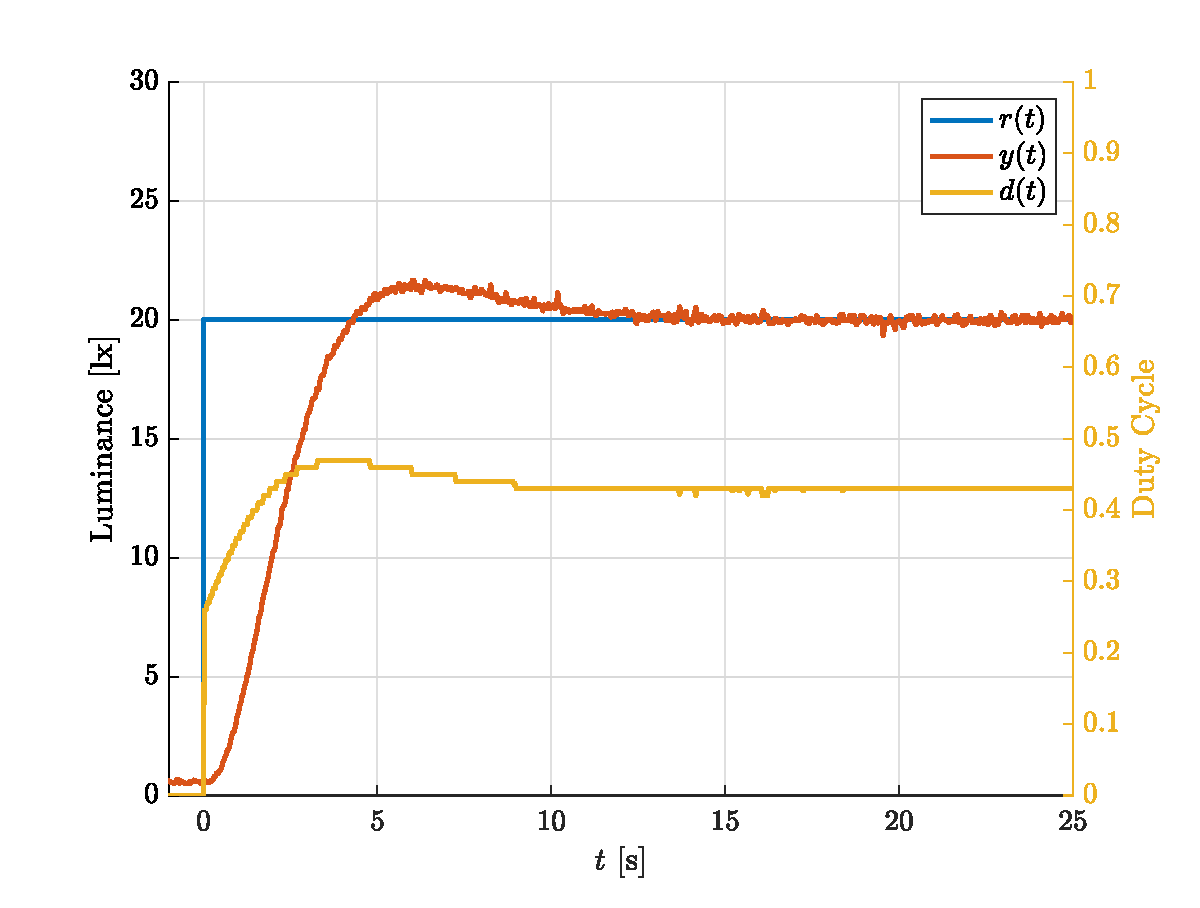
\includegraphics[width=\linewidth]{Imagens/Subimage2.eps}
        \caption{Subfigura 2}
        \label{fig:2.2}
    \end{subfigure}%
    \begin{subfigure}{0.33\textwidth}
        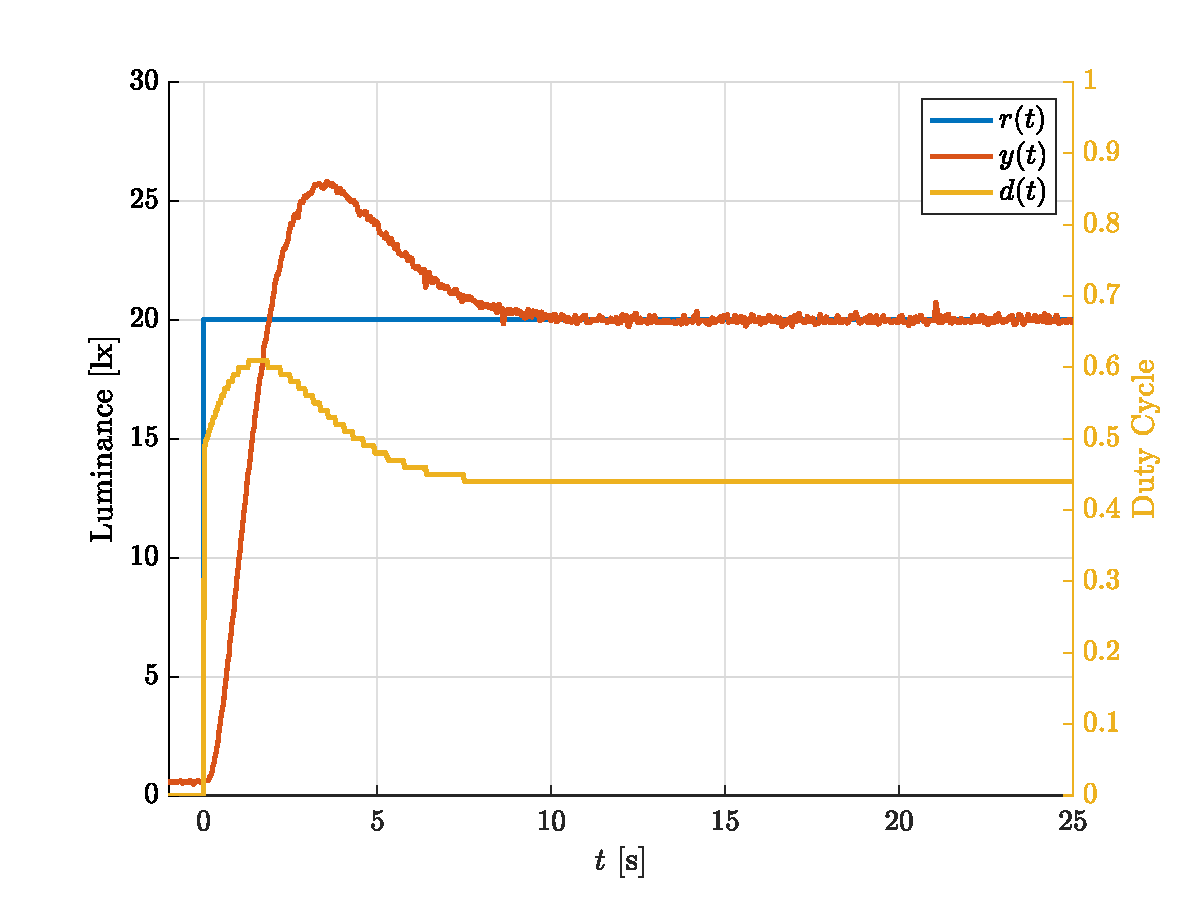
\includegraphics[width=\linewidth]{Imagens/Subimage3.eps}
        \caption{Subfigura 3}
        \label{fig:2.3}
    \end{subfigure}
    \caption{Descrição da imagem}
    \label{fig:2}
\end{figure}

\subsection{Task 2}


\subsection{Task 3}


\subsection{Task 4}

To reconstruct the sensor orientation in Euler angles \((\alpha, \beta, \gamma)\) using rate-gyro data, we analyze the relationship between angular velocities \((\omega_x, \omega_y, \omega_z)\) and the derivatives of the Euler angles. The \textbf{ZYX Euler angle convention} was selected because it provides an intuitive sequence for controlling robotic manipulators, such as the Scorbot VII, allowing separate adjustments for direction, height, and tool orientation.

\subsubsection{Theory and Mathematical Formulation}

In this convention, the angles represent rotations applied in a specific order:
\begin{itemize}
    \item \textbf{Yaw (\(\gamma\))} — rotation about the global Z-axis. This initial rotation aligns the manipulator to face the target, orienting its base towards the goal.
    \item \textbf{Pitch (\(\beta\))} — rotation about the new Y-axis after the yaw rotation. This step adjusts the vertical alignment of the manipulator relative to the goal.
    \item \textbf{Roll (\(\alpha\))} — rotation about the new X-axis following the yaw and pitch rotations. This final adjustment ensures the gripper or tool is properly oriented for interaction with the target.
\end{itemize}

By properly parameterizing these rotations, we ensure predictable and precise control of the manipulator's movements, essential for tasks involving accurate positioning and end-effector orientation.

\paragraph{Parameterization}
To reconstruct the orientation accurately, we define the following parameters:
\begin{itemize}
    \item \(\alpha, \beta, \gamma\): Euler angles representing the sensor's orientation in 3D space.
    \item \(\omega_x, \omega_y, \omega_z\): Angular velocities provided by the rate-gyro, indicating rotational speeds around the sensor’s local axes. These values are taken from the dataset provided in the file.
    \item \(\Delta t\): Time interval between consecutive measurements, essential for discrete numerical integration.
    \item \(\mathbf{J}(\alpha, \beta, \gamma)\): Jacobian matrix that relates the angular velocities to the changes in the Euler angles.
\end{itemize}

The task is to relate the angular velocities \((\omega_x, \omega_y, \omega_z)\) to the time derivatives of the Euler angles \((\dot{\alpha}, \dot{\beta}, \dot{\gamma})\), using a transformation matrix.

The relationship between angular velocities and the derivatives of the Euler angles is defined by the Jacobian matrix, shown in Equation~\eqref{eq:jacobian_relationship}:

\begin{equation}
\label{eq:jacobian_relationship}
\begin{bmatrix}
\dot{\alpha} \\
\dot{\beta} \\
\dot{\gamma}
\end{bmatrix} = 
\mathbf{J}^{-1}(\alpha, \beta, \gamma) \cdot 
\begin{bmatrix}
\omega_x \\
\omega_y \\
\omega_z
\end{bmatrix}
\end{equation}

Where \( \mathbf{J}(\alpha, \beta, \gamma) \) is the Jacobian matrix that links the angular velocities to the changes in Euler angles. For the ZYX convention, the Jacobian matrix is given by Equation~\eqref{eq:jacobian_matrix}:

\begin{equation}
\label{eq:jacobian_matrix}
\mathbf{J}(\alpha, \beta) =
\begin{bmatrix}
1 & \sin(\alpha) \tan(\beta) & \cos(\alpha) \tan(\beta) \\
0 & \cos(\alpha) & -\sin(\alpha) \\
0 & \frac{\sin(\alpha)}{\cos(\beta)} & \frac{\cos(\alpha)}{\cos(\beta)}
\end{bmatrix}
\end{equation}

Each term in the Jacobian matrix reflects the dependency between rotations and angular velocities. For instance, the appearance of trigonometric functions, such as \(\sin(\alpha)\) or \(\cos(\beta)\), results from the sequential nature of the ZYX rotations and their cumulative impact on the orientation.

From this matrix, we derive the equations for the time derivatives of the Euler angles, presented in Equations~\eqref{eq:alpha_dot}, \eqref{eq:beta_dot}, and \eqref{eq:gamma_dot}:

\begin{equation}
\label{eq:alpha_dot}
\dot{\alpha} = \omega_x + \sin(\alpha) \tan(\beta) \cdot \omega_y + \cos(\alpha) \tan(\beta) \cdot \omega_z
\end{equation}

\begin{equation}
\label{eq:beta_dot}
\dot{\beta} = \cos(\alpha) \cdot \omega_y - \sin(\alpha) \cdot \omega_z
\end{equation}

\begin{equation}
\label{eq:gamma_dot}
\dot{\gamma} = \frac{\sin(\alpha)}{\cos(\beta)} \cdot \omega_y + \frac{\cos(\alpha)}{\cos(\beta)} \cdot \omega_z
\end{equation}

\paragraph{Example Calculation}
To illustrate the use of these formulas with real data, consider an entry from the dataset provided in the file. For the time step corresponding to \( t = 692028 \, \mu s \), the rate-gyro measurements are:

\begin{equation}
\label{eq:rate-gyro}
\omega_x = -2.0^\circ/\text{s}, \quad \omega_y = 1.0^\circ/\text{s}, \quad \omega_z = -1.0^\circ/\text{s}
\end{equation}

We convert them to radians per second:

\begin{equation}
\label{eq:rate-gyro-rad}
\omega_x \approx -0.0349 \, \text{rad/s}, \quad \omega_y \approx 0.0175 \, \text{rad/s}, \quad \omega_z \approx -0.0175 \, \text{rad/s}
\end{equation}

For the initial conditions, let's assume the current Euler angles are all zero:
\[
\alpha_k = 0.0 \, \text{rad}, \quad \beta_k = 0.0 \, \text{rad}, \quad \gamma_k = 0.0 \, \text{rad}
\]

We can calculate the derivatives using Equations~\eqref{eq:alpha_dot}, \eqref{eq:beta_dot}, and \eqref{eq:gamma_dot}:

\[
\dot{\alpha}_k = -0.0349 + \sin(0.0) \cdot \tan(0.0) \cdot 0.0175 + \cos(0.0) \cdot \tan(0.0) \cdot (-0.0175)
\]
\[
\dot{\beta}_k = \cos(0.0) \cdot 0.0175 - \sin(0.0) \cdot (-0.0175) = 0.0175
\]
\[
\dot{\gamma}_k = \frac{\sin(0.0)}{\cos(0.0)} \cdot 0.0175 + \frac{\cos(0.0)}{\cos(0.0)} \cdot (-0.0175) = -0.0175
\]

After calculating the derivatives, they are:
\[
\dot{\alpha}_k \approx -0.0349 \, \text{rad/s}, \quad \dot{\beta}_k \approx 0.0175 \, \text{rad/s}, \quad \dot{\gamma}_k \approx -0.0175 \, \text{rad/s}
\]

These derivatives will then be integrated over time to estimate the updated Euler angles.

\subsubsection{Numerical Integration}
To estimate the Euler angles over time, numerical integration is performed using the angular velocities. The continuous integration formulas are given in Equations~\eqref{eq:alpha_integral}, \eqref{eq:beta_integral}, and \eqref{eq:gamma_integral}:

\begin{equation}
\label{eq:alpha_integral}
\alpha(t) = \alpha_0 + \int_0^t \dot{\alpha} \, dt
\end{equation}

\begin{equation}
\label{eq:beta_integral}
\beta(t) = \beta_0 + \int_0^t \dot{\beta} \, dt
\end{equation}

\begin{equation}
\label{eq:gamma_integral}
\gamma(t) = \gamma_0 + \int_0^t \dot{\gamma} \, dt
\end{equation}

For discrete time intervals, the equations become:

\begin{equation}
\label{eq:alpha_discrete}
\alpha_{k+1} = \alpha_k + \dot{\alpha}_k \cdot \Delta t
\end{equation}

\begin{equation}
\label{eq:beta_discrete}
\beta_{k+1} = \beta_k + \dot{\beta}_k \cdot \Delta t
\end{equation}

\begin{equation}
\label{eq:gamma_discrete}
\gamma_{k+1} = \gamma_k + \dot{\gamma}_k \cdot \Delta t
\end{equation}

Here, \( \Delta t \) is the time interval between consecutive measurements.



% ----------------------------------------------------------------------
% Conclusão
% ----------------------------------------------------------------------
\section{Conclusion}

\lipsum[1] \cite{refs1, refs2, refs3}

% ----------------------------------------------------------------------
% Referências
% ----------------------------------------------------------------------
\bibliographystyle{plain}
\bibliography{refs}

% ----------------------------------------------------------------------
% Apêndices
% ----------------------------------------------------------------------
\appendix  
\clearpage
\addappheadtotoc 
\appendixpage 

\section{First Appendix}

\lipsum[1]

\section{Segundo anexo}

\lipsum[1]
\end{document}